\documentclass[../main]{subfiles}
\begin{document}
\section{La ecuación Geodésica}

En Relatividad General tenemos dos ideas clave: 
\begin{enumerate}
    \item La curvatura del espacio-tiempo le ``dice'' a la materia como moverse.
    \item La materia dictamina como el espacio-tiempo debe curvarse.
\end{enumerate}

\section{Acción de una partícula puntual}

La acción de una partícula puntual relativista está dada por:
\begin{equation}
    S=-m \int \mathrm{d}\tau
\end{equation}
donde $\tau$ es el tiempo propio. 

\textcolor{red}{Check 1:} En Minkowski tenemos: 
\begin{equation}
    \begin{split}
        \mathrm{d}\tau&=\sqrt{\mathrm{d}t^2-\mathrm{d}\vec{x}^2}\\
        &=\mathrm{d}t\sqrt{1-\left(\dv{x}{t}\right)^2} \\
        &=\mathrm{d}t\sqrt{1-v^2}
    \end{split}
\end{equation}

Y en nuestra acción, tenemos 
\begin{equation}
    \begin{split}
        S&=-m \int \mathrm{d}t\sqrt{1-v^2},\quad v<<1 \\
        &=\int \mathrm{d}t\left(-m+\dfrac{1}{2}mv^2+\Phi\right)        
    \end{split}
\end{equation}

\textcolor{red}{Check 2:} Usando la métrica de campo débil
\begin{equation}
    ds^2=-(1+2\Phi(x))\mathrm{d}t^2+(1-2\Phi)\mathrm{d}\vec{x}^2,\quad \Phi<<1,
\end{equation}
tenemos:
\begin{equation}
    \begin{split}
        S&=-m\int \mathrm{d}t \sqrt{(1+2\Phi)-(1-2\Phi)V^2} \\
        S&\sim \int \mathrm{d}\tau \left(-m+\dfrac{1}{2}mV^2+m\Phi+\cdots \Theta(\Phi^2)\right) 
    \end{split}
\end{equation}

\section{La ecuación geodésica}
Considere una curva $x^{\mu}(\lambda)$ en un espacio-tiempo general con métrica $g_{\mu\nu}(t, \vec{x})$:
\begin{center}
    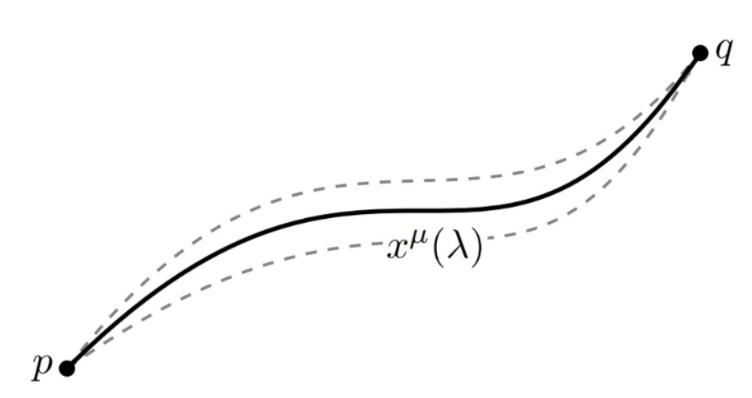
\includegraphics[scale=0.5]{img/imgRG3.1.PNG}
\end{center}
\definicion{} La geodésica es la curva preferida para la cual la acción es un extremo ($\delta S=0$):
\begin{equation}
    \dv{^2 x^{\mu}}{\lambda^2}+\Gamma^{\mu}_{\alpha\beta}\dv{x^{\alpha}}{\lambda}\dv{x^{\beta}}{\lambda}=0
\end{equation}
donde $\Gamma^{\mu}_{\alpha\beta}$ es el símbolo de Christoffel:
\begin{equation}
    \Gamma^{\mu}_{\alpha\beta}=\dfrac{1}{2}g^{\mu\lambda}(\partial_{\alpha}g_{\beta\lambda}+\partial_{\beta}g_{\alpha\lambda}-\partial_{\lambda}g_{\alpha\beta})
\end{equation}
donde $\partial_{\alpha}$ es la derivada parcial respecto a las coordenadas contravariantes $x^{\alpha}$:
\begin{equation}
    \partial_{\alpha} \rightarrow \pdv{}{x^{\alpha}}
\end{equation}

\textcolor{red}{Demostración:} Para una métrica general $g_{\mu\nu}$, la acción $S[x^{\mu}(\lambda)]$, viene dada por:
\begin{equation}
    S[x^{\mu}(\lambda)]=-m\int \mathrm{d}\lambda \sqrt{-g_{\mu\nu}\dv{x^{\mu}}{\lambda}\dv{x^{\nu}}{\lambda}}
\end{equation}
considerando $x^{\mu} \ \rightarrow \ x^{\mu}+\delta x^{\mu}$ tal que $\delta S=S[x^{\mu}+\delta x^{\mu}]-S[x^{\mu}]$ tenemos que $\delta S=0$ para cualquier $\delta x^{\mu}$ sí:
\begin{equation}
    \begin{split}
        \delta \int \mathrm{d}\tau&=\dfrac{1}{2}\int \mathrm{d}\lambda \left(-g_{\mu\nu}\dv{x^{\mu}}{\lambda}\dv{x^{\nu}}{\lambda}\right)^{-1/2} \left[-\delta g_{\mu\nu} \dv{x^{\mu}}{\lambda}\dv{x^{\nu}}{\lambda}-2g_{\mu\nu}\dv{\delta x^{\mu}}{\lambda}\dv{x^{\nu}}{\lambda}\right]\\
        \delta S&=\dfrac{1}{2}\int \mathrm{d} \lambda \left\{-\partial_{\lambda}g_{\mu\nu}\dot{x}^{\mu}\dot{x}^{\nu}\delta x^{\lambda}+2g_{\mu\nu}\ddot{x}^{\nu}\delta x^{\mu}+\partial_{\lambda}g_{\mu\nu}\dot{x}^{\lambda}\dot{x}^{\nu}\delta x^{\mu} \right\}
    \end{split}
\end{equation}

Donde hemos usado la propiedad: $\delta g_{\mu\nu}=\partial_{\lambda}g_{\mu\nu}\delta x^{\lambda}$
\begin{equation}
    \delta S=\int \mathrm{d}\lambda \left\{g_{\mu\nu}\ddot{x}^{\nu}+\dfrac{1}{2}\left(\partial_{\lambda}g_{\mu\nu}+\partial_{\nu}g_{\mu\lambda}-\partial_{\mu}g_{\nu\lambda}\right)+\dot{x}^{\nu}\dot{x}^{\lambda} \right\}\delta x^{\mu}=0\\
\end{equation}
escribiendo $\Gamma^{\mu}_{\nu\lambda}=\dfrac{1}{2}g^{\mu\rho}\left(\partial_{\lambda}g_{\rho\nu}+\partial_{\nu}g_{\rho\lambda}-\partial_{\rho}g_{\nu\lambda}\right)$:
\begin{equation}
    \delta S=\int \mathrm{d}\lambda g_{\mu\nu}\left(\ddot{x}^{\nu}+\Gamma^{\nu}_{\rho\lambda}\dot{x}^{\rho}\dot{x}^{\lambda}\right)\delta x^{\mu}=0\\
\end{equation}
para variaciones arbitrarias $\delta x^{\mu}$; $\delta S=0$:
\begin{equation}
    \dv{^2 x^{\nu}}{\tau^2}+\Gamma^{\nu}_{\rho\lambda}\dv{x^{\rho}}{\tau}\dv{x^{\lambda}}{\tau}=0
\end{equation}
obtenemos la ecuación geodésica.

Nota: Observe que la misma ecuación geodésica puede ser derivada del lagrangiano:
\begin{equation}
    L=-g_{\mu\nu} \dv{x^{\mu}}{\lambda} \dv{x^{\nu}}{\lambda}
    \label{ec3.14}
\end{equation}

\section{Cantidades conservadas}
Si $L$ no depende explicitamente de $\lambda$ tal que $\pdv{L}{\lambda}=0$, luego: 
\begin{equation}
    \begin{split}
        \dv{L}{\lambda}&=\pdv{L}{\lambda}+\dv{x^{\mu}}{\lambda}\pdv{L}{x^{\mu}}+\dv{\dot{x}^{\mu}}{\lambda}\pdv{L}{\dot{x}^{\mu}}\\
        \dv{L}{\lambda}&=\dot{x}^{\mu}\dv{}{\lambda}\left(\pdv{L}{\dot{x}^{\mu}}\right)+\dv{\dot{x}^{\mu}}{\lambda}\pdv{L}{\dot{x}^{\mu}}\\
        \dv{L}{\lambda}&=\dv{}{\lambda}\left(\pdv{L}{\dot{x}^{\mu}}\dot{x}^{\mu}\right)\\
        0&=\dv{}{\lambda}\left(L-\pdv{L}{\dot{x}^{\mu}}\dot{x}^{\mu}\right)
    \end{split}
\end{equation}
De la conservación de la energía, tenemos:
\begin{equation}
    H=L-\pdv{L}{\dot{x}^{\mu}}\dot{x}^{\mu} \quad \rightarrow \quad H=-g_{\mu\nu}\dv{x^{\mu}}{\lambda}\dv{x^{\nu}}{\lambda}
\end{equation}

Si $g_{\mu\nu}$ no depende de alguna coordenada, luego $\partial_{\alpha}g_{\mu\nu}=0$ las ecuaciones de Euler-Lagrange:
\begin{equation}
    \begin{split}
        \dv{}{\lambda}\left(\pdv{L}{\dot{x}^{\alpha}}\right)-\pdv{L}{x^{\alpha}}&=0\\
        \dv{}{\lambda}\left(-2g_{\alpha\nu}\dv{x^{\nu}}{\lambda}\right)&=-\underbrace{\partial_{\alpha}g_{\mu\nu}}_{0} \dv{x^{\mu}}{\lambda}\dv{x^{\nu}}{\lambda}\\
        \dv{}{\lambda}\left(-2g_{\alpha\nu}\dv{x^{\nu}}{\lambda}\right)&=0
    \end{split}
\end{equation}

La cantidad $-2g_{\alpha\nu}\dv{x^{\nu}}{\lambda}=Const$ corresponde al momento conjugado a la coordenada $x^{\alpha}$.

\section{El límite Newtoniano}

Condiciones:
\begin{enumerate}
    \item Partículas moviendose lentamente.
    \item El campo gravitacional es débil.
    \item El campo es estático.
\end{enumerate}

\begin{enumerate}
    \item Para partículas $v<<1$ la ecuación geodésica:
    \begin{equation}
        \dv{^2 x^{\mu}}{\tau^2}+\Gamma^{\mu}_{00}\left(\dv{t}{\tau}\right)^2=0
    \end{equation}
    \item Implica que $g_{\mu\nu}=\eta_{\mu\nu}+h_{\mu\nu}$; $g^{\mu\nu}=\eta^{\mu\nu}-h^{\mu\nu}$ donde $|h_{\mu\nu}|<<1$. A primer orden en $h_{\mu\nu}$, tenemos:
    \begin{equation}
        \Gamma^{\mu}_{00}=\dfrac{1}{2}g^{\mu\lambda}(\partial_0 g_{0\lambda}+\partial_0 g_{0\lambda}-\partial_{\lambda}g_{00})=\dfrac{1}{2}\eta^{\mu j}\partial_j h_00
    \end{equation}
    Para $\mu=0$ la ecuación geodésica nos queda:
    \begin{equation}
        \dv{^2 t}{\tau^2}=0 \quad \rightarrow \quad \dv{t}{\tau}=cte
    \end{equation}
    Para $\mu=i$ se tiene que:
    \begin{equation}
        \dv{^2 x^{i}}{\tau^2}=\dfrac{1}{2}\partial^{i}h_{00}\left(\dv{t}{\tau}\right)^2,
    \end{equation}
    donde al transformar $\tau \rightarrow t$ y definiendo $h_{00}=-2\Phi$, se tiene que:
    \begin{equation}
        \dv{^2 x^{i}}{t^2}=-\partial^{i}\Phi
    \end{equation}
    En coordenadas contravariantes $x^{i}:\partial_i \rightarrow \vec{\nabla}$, a primer orden en $h$:
    \begin{equation}
        \dv{^2 \vec{x}}{t^2}=-\vec{\nabla}\Phi
    \end{equation}
\end{enumerate}
\section{Geodésicas en la métrica de Schwarzschild}
La métrica alrededor de un objeto de masa $M$ viene dada por:
\begin{equation}
    \mathrm{d}s^2=-\left(1-\dfrac{2GM}{r}\right)\mathrm{d}t^2+\left(1-\dfrac{2GM}{r}\right)^{-1}\mathrm{d}r^2+r^2(\mathrm{d}\theta^2+\sin^2 \theta \mathrm{d}\phi^2)
\end{equation}
de donde podemos extraer las cantidades conservadas para este espacio-tiempo usando el lagrangiano en \eqref{ec3.14}
\begin{equation}
    L=\left(1-\dfrac{2GM}{r}\right)\dot{t}^2-\left(1-\dfrac{2GM}{r}\right)^{-1}\dot{r}^2-r^2\mathrm{d}\dot{\theta}^2-r^2\sin^2 \theta \mathrm{d}\dot{\phi}^2
\end{equation}

La ecuación de Euler-Lagrange
\begin{equation}
    \dv{}{\lambda}\left(\pdv{L}{\dot{x}^{\mu}}\right)-\pdv{L}{x^{\mu}}=0, \ x^{\mu}\rightarrow 
    \left\{
    \begin{array}{c}
       t\\
       r\\
       \theta\\
       \phi 
    \end{array}
    \right.
\end{equation}

Dado que el lagrangiano $L$ no depende explícitamente de $t$ y $\phi$, se sigue que:
\begin{align}
    \dv{}{\lambda}\left(\pdv{L}{\dot{t}}\right)&=0 \quad \rightarrow \quad E=\dfrac{1}{2}\pdv{L}{\dot{t}}=\left(1-\dfrac{2GM}{r}\right)\dot{t}  &(\text{Energía})\\
    \dv{}{\lambda}\left(\pdv{L}{\dot{\phi}}\right)&=0 \quad \rightarrow \quad L=-\dfrac{1}{2}\pdv{L}{\dot{\phi}}=r^2\sin^2 \theta \dot{\phi}  &(L_z) 
\end{align}
Nótese que estas definiciones deben concordar con las de mecánica clásica.

La ecuación para $\theta$ viene dada por:
\begin{equation}
    \dv{}{\lambda}(r^2 \dot{\theta})=r^2\sin \theta \cos \theta \dot{\phi}^2 \quad \rightarrow \quad \ddot{\theta}=\dfrac{\cos \theta}{\sin^3 \theta} \dfrac{L^2}{r^4}-2\dfrac{\dot{r}}{r}\dot{\theta}
\end{equation}

Esta ecuación para $\theta=\pi/2$(plano ecuatorial) y $L=\epsilon$ constante se tiene que:
\begin{equation}
    \epsilon=\left(1-\dfrac{2GM}{r}\right)\dot{t}^2-\left(1-\dfrac{2GM}{r}\right)^{-1}\dot{r}^2-r^2\dot{\phi}^2=
    \left\{
    \begin{array}{cc}
        +1 & \text{timelike}\\
        0  & \text{Null}
    \end{array}
    \right.
\end{equation}
usando las cantidades conservadas:
\begin{equation}
    \epsilon = \left(1-\dfrac{2GM}{r}\right)^{-1} E^2-\left(1-\dfrac{2GM}{r}\right)^{-1}\dot{r}^2-\dfrac{L^2}{r^2},
\end{equation}
esto es:
\begin{equation}
    -E^2+\dot{r}^2+\left(1-\dfrac{2GM}{r}\right)\left(\dfrac{L^2}{r^2}+\epsilon\right)=0
\end{equation}
esta ecuación puede ser escrita como:
\begin{equation}
    \dfrac{1}{2}\dot{r}^2+V(r)=\epsilon
\end{equation}
donde $\epsilon=E^2/2$ y $V(r)$ es el potencial efectivo:
\begin{equation}
    V(r)=\epsilon\dfrac{c^2}{2}+\epsilon\dfrac{GM}{r}+\dfrac{L^2}{2r^2}-\dfrac{L^2 GM}{c^2 r^3}
\end{equation}
donde $\dfrac{GM}{r}$ es potencial Newtoniano, $\dfrac{L^2}{2r^2}$ es el potencial centrífugo y $\dfrac{L^2 GM}{c^2 r^3}$ es la correción de la relatividad general.
\section{Orbitas Circulares}

Una partícula puede moverse en una orbita circular $r=r_c$ cuando $\mathrm{d}V/\mathrm{d}r=0$.
\begin{enumerate}
    \item Partículas sin masa $(\epsilon=0)$
    \begin{equation}
        V(r)=\dfrac{L^2}{2r^2}-\dfrac{L^2 GM}{r^3} \ \rightarrow \ \dv{V}{r}=-\dfrac{L^2}{r^3}+\dfrac{3L^2 GM}{r^4}=0
    \end{equation}
    donde $r_c=3GM$ (Photon Sphere).

    Nota: No hay órbitas circulares para partículas en gravedad Newtoniana. La evolución depende de como $\epsilon$ se compara con $V_{max}=V(r_c)$:
    \begin{itemize}
        \item Para $\epsilon<V_{max}$, la luz emitida en $r<r_c$ no puede escapar a infinito, mientras que para $r>>r_c$ la luz rebota en la barrera de potencial de momento angular regresando a infinito.
        \item Para $\epsilon>V_{max}$, la energía es mayor que la barrera de potencial de momento angular. En este caso la luz emitida en $r<r_c$ puede escapar, mientras que para la luz emitida desde $r>>r_c$ pueden alcanzar $r=0$.
    \end{itemize}
    \item Partículas con masa $(\epsilon=1)$
    \begin{equation}
        V(r)=\dfrac{1}{2}-\dfrac{GM}{r}+\dfrac{L^2}{2r^2}-\dfrac{L^2 GM}{r^3} \ \rightarrow \ \dv{V}{r}=\dfrac{GM}{r^2}-\dfrac{L^2}{r^3}+\dfrac{3L^2 GM}{r^4}=0
    \end{equation}
    entonces 
    \begin{equation}
        GMr^2_c-L^2 r_c+3GML^2=0,\quad r_c(L)_{\pm}=\dfrac{L^2 \pm \sqrt{L^4-12(GM)^2L^2}}{2GM}
    \end{equation}
    Las soluciones dependen de $L^2$

    \begin{minipage}{0.5\textwidth}
        \begin{center}
            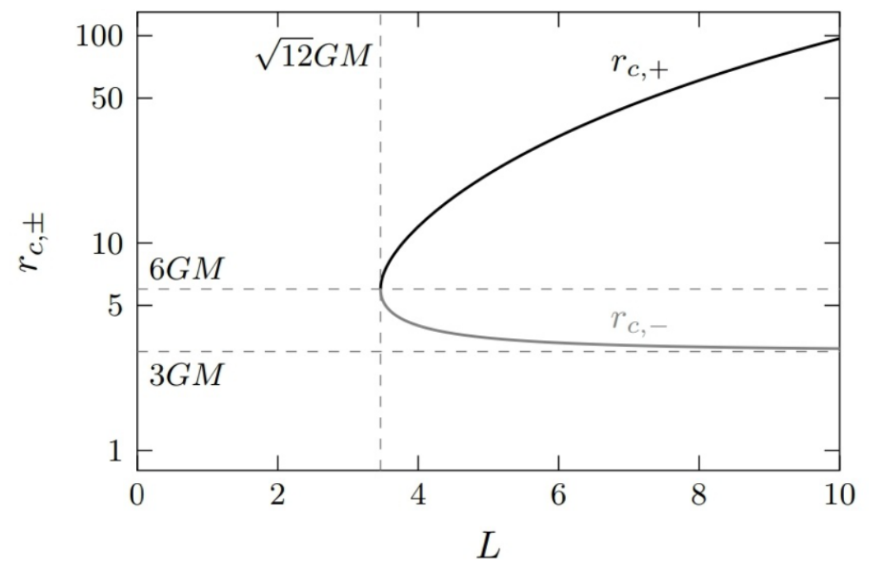
\includegraphics[scale=0.37]{img/imgRG3.2.PNG}
        \end{center}
    \end{minipage}
    \begin{minipage}{0.5\textwidth}
        \begin{itemize}
            \item Para $L>\sqrt{12}GM$ órbitas estables $r_{c,+}$ inestables $r_{c,-}$.
            \item Para $L=\sqrt{12}GM$ las dos soluciones se reducen a una órbita $r_c=6GM$.
            \item Para $L<\sqrt{12}GM$ no hay órbitas circulares estables.
        \end{itemize}
    \end{minipage}
\end{enumerate}
\section{Precesión de la órbita de Mercurio}

La Relatividad General explica la precesión del perihelio del Mercurio.
\begin{center}
    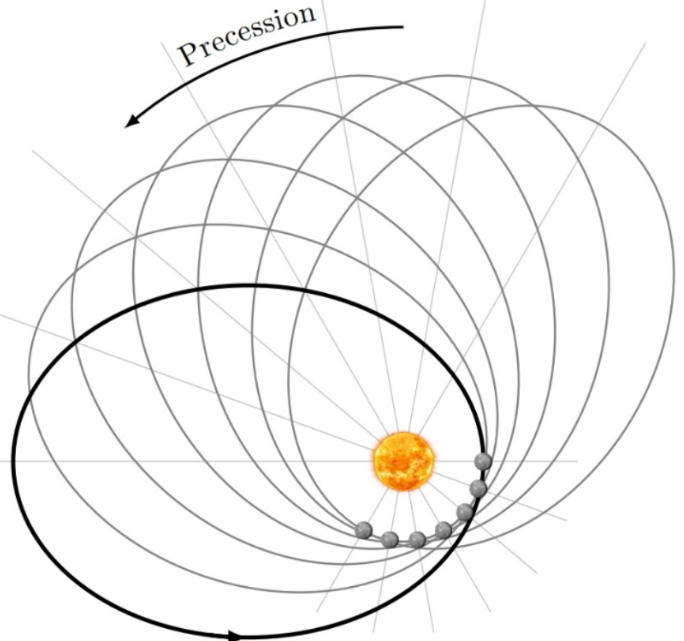
\includegraphics[scale=0.5]{img/imgRG3.3.PNG}
\end{center}

Para demostrar como $r$ es función de $\phi$, usamos:
\begin{equation}
    \dfrac{1}{2}\left(\dv{r}{\lambda}\right)^2+\left(\dfrac{1}{2}-\dfrac{GM}{r}+\dfrac{L^2}{2r^2}-\dfrac{L^2 GM}{r^3}\right)=\epsilon
    \label{ec3.38}
\end{equation}
usando la regla de cadena:
\begin{equation}
    \left(\dv{r}{\lambda}\right)^2=\left(\dv{\phi}{\lambda}\right)^2\left(\dv{r}{\phi}\right)^2=\dfrac{L^2}{r^4}\left(\dv{r}{\phi}\right)^2
\end{equation}
de donde la ecuación \eqref{ec3.38} puede ser reescrita como:
\begin{equation}
    \left(\dv{r}{\phi}\right)^2+\dfrac{r^4}{L^2}-\dfrac{2GM}{L^2}r^3+r^2-2GMr=\dfrac{2\epsilon r^4}{L^2}
\end{equation}
cambiando variables $u=\dfrac{L^2}{GMr}$, donde $u=1$ para una órbita circular:
\begin{equation}
    \left(\dv{u}{\phi}\right)^2+\dfrac{L^2}{(GM)^2}-2u+u^2-\dfrac{2(GM)^2 u^3}{L^2}=\dfrac{2\epsilon L^2}{(GM)^2}
\end{equation}

Derivando respecto a $\phi$:
\begin{equation}
    \dv{^2 u}{\phi^2}-1+u=\dfrac{3(GM)^2 u^2}{L^2}
\end{equation}

Que tiene la siguiente solución particular:
\begin{equation}
    u_1=\dfrac{3(GM)^2}{L^2}\left[\left(1+\dfrac{1}{2}e^2\right)+e\phi\sin \phi-\dfrac{1}{6}e^2\cos(2\phi)\right]
\end{equation}

Tenemos que:
\begin{equation}
    \begin{split}
        u&=1+e\cos \phi+\alpha e\phi \sin\phi \ \rightarrow \ \alpha=\dfrac{3(GM)^2}{L^2}<<1\\
        u&\simeq 1+e\cos\left[(1-\alpha)\phi\right]
    \end{split}
\end{equation}

Durante cada orbita, el perihelio cambia $\Delta \phi$ dado por:
\begin{equation}
    \Delta \phi=2\pi \alpha=6\pi\dfrac{(GM)^2}{L^2}
\end{equation}
para una orbita elíptica $L^2 \simeq GM(1-e^2)a$
\begin{equation}
    \Delta \phi = \dfrac{6\pi GM}{c^2(1-e^2)a}
\end{equation}

Para Mercurio, los parámetros relevantes:
\begin{equation}
    \begin{split}
        GM_0=1.48\times 10^3 \text{m},\quad a=5.79\times 10^{10}\text{m},\quad e=0.2056\\
        \Delta \phi_{mercurio}=5.01\times 10^{-7} rad/orbita=0.103''/orbita 
    \end{split}
\end{equation}
Usando $T=88$ días y $\Delta \phi_{mercurio}=43.0''/siglo$, la precesión observada restando los efectos gravitacionales de los demás planetas es 
\begin{equation}
    \Delta \phi_{mercurio}-532''/siglo\approx 43''/siglo
\end{equation}

\section{Bending of Light}

La primera evidencia experimental de la validez para GR provino de la desviación de la luz de las estrellas de fondo por el sol.

Para Schwarzschild tenemos la ecuación radial:
\begin{equation}
    \dfrac{1}{2}\dot{r}^2+\dfrac{L^2}{2r^2}\left(1-\dfrac{2GM}{r}\right)=\dfrac{E^2}{2}
\end{equation}
\begin{center}
    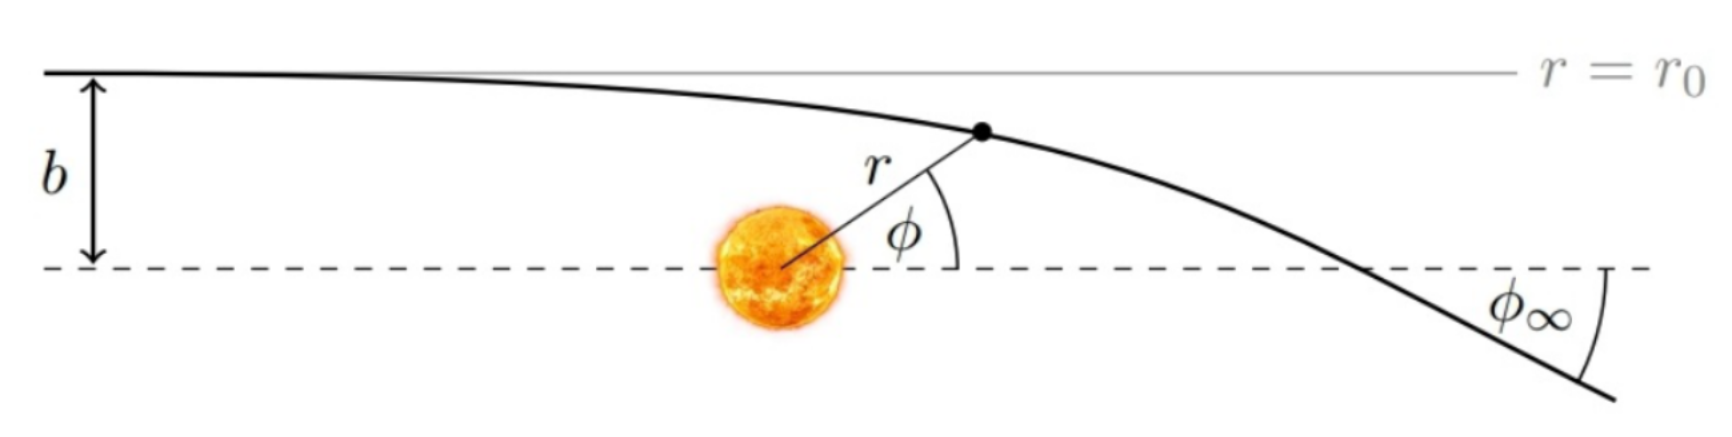
\includegraphics[scale=0.3]{img/imgRG3.4.PNG}
\end{center}

Cambiando variables $u=1/r$ obtenemos la siguiente ecuación diferencial no homogénea
\begin{equation}
    \dv{^2 u}{\phi^2}+u=3GM u^2
\end{equation}
entonces 
\begin{equation}
    u=\dfrac{1}{b}\sin \phi+\dfrac{GM}{2b^2}(3+4\cos \phi+\cos (2\phi))
\end{equation}

Para $\phi_{\infty}$ la luz escapa $r=\infty$ ($u=0$) asumiendo que la desviación es pequeña 
\begin{equation}
    \phi_{\infty}\approx -\dfrac{4GM}{bc^2} \quad \text{para el sol} \quad b\approx R_{\odot}
\end{equation}
y también el observado por Eddington en 1919
\begin{equation}
    \phi_{\infty}\approx 8.6\times 10^{-5}rad \simeq 18''
\end{equation}

\section*{Problemas 3}

\begin{enumerate}
    \item \textbf{Derivada Covariante}
    \begin{enumerate}[label=(\alph*)]
        \item Sea 
        \begin{equation}
            T^{j_1 \cdots j_s}_{i_1 \cdots i_r}\mathrm{d}x^{i_1} \otimes \cdots \otimes \mathrm{d}x^{i_r}\otimes \pdv{}{x^{j_1}} \otimes \cdots \otimes \pdv{}{x^{j_s}}. 
        \end{equation}
        Entonces, $\nabla T$ puede ser escrito localmente por 
        \begin{equation}
            \nabla T=W^{j_1 \cdots j_s}_{i_1 \cdots i_r} \mathrm{d}x^{i} \otimes \mathrm{d}x^{i_1} \otimes \cdots \otimes \mathrm{d}x^{i_r} \otimes \pdv{}{x^{j_1}} \otimes \cdots \otimes \pdv{}{x^{j_s}}.
        \end{equation}
        Demostrar que 
        \begin{equation}
            W^{j_1 \cdots j_s}_{i_1 \cdots i_r}=\pdv{T^{j_1 \cdots j_s}_{i_1 \cdots i_r}}{x^{i}}+\sum_{m=1}^s \Gamma^{jm}_{iq} T^{j_1 \cdots j_{m-1}qj_m \cdots j_s}_{i_1 \cdots i_r}-\sum_{\ell=1}^r \Gamma^{p}_{iil}T^{j_1 \cdots j_s}_{i_1 \cdots i_{\ell}}
        \end{equation}
        \item Si escribimos $g=g_{ij}\mathrm{d}x^{i}\otimes \mathrm{d}x^{j}$, la métrica inducida sobre $T^* M$ es denotada por $g^{-1}=g^{ij}\pdv{}{x^{i}}\otimes \pdv{}{x^{j}}$ donde $(g^{ij})$ es la matriz inversa de $(g_{ij})$. Entonces, existe una métrica inducida sobre $T^* M\otimes T^* M$ y la denotamos por $g$. Es decir, si $S=S_{ij}\mathrm{d}x^{i}\otimes \mathrm{d}x^{j}$ y $T=T_{kl}\mathrm{d}x^k \otimes \mathrm{d}x^{\ell}$, entonces su producto interno es definido como 
        \begin{equation}
            \langle S, T \rangle_g = g(S, T)=S_{ij} T_{k\ell} g\left(\mathrm{d}x^{i}\otimes \mathrm{d}x^{j}, \mathrm{d}x^k\otimes \mathrm{d}x^{\ell}\right)=g^{ik}g^{j\ell} S_{ij}T_{k\ell}.
        \end{equation}
        Para cualquier tensor $T \in Gamma(M, T^* M\otimes T^* M)$, el operador \textit{traza} es definido como 
        \begin{equation}
            \tr_g T:=g^{ij}T_{ij}
        \end{equation}
        Para cualquier $S, T \in Gamma(M, T^* M \otimes T^* M)$ y $X \in \Gamma(M, TM)$, demostrar que 
        \begin{equation}
            X(g(S, T))=g(\nabla_X S, T)+g(S, \nabla_X T).
        \end{equation}
        En particular, si $S=g$, demostrar que 
        \begin{equation}
            X(\tr_g T)=\langle g, \nabla_X T\rangle_g.
        \end{equation}
        Localmente es 
        \begin{equation}
            \nabla_{\pdv{}{x^{i}}}(\tr_g T)=\nabla_{\pdv{}{x^{i}}}\left(g^{k\ell} T_{k\ell}\right)=g^{k\ell}(\nabla_i T_{k\ell})
        \end{equation}
        \item Sea $\mathrm{d}vol=\sqrt{\det (g_{mn})}\mathrm{d}x^1 \cdots \mathrm{d}x^n$ la forma de volumen. Demuestre que 
        \begin{equation}
            \pdv{\sqrt{\det(g_{mn})}}{x^{j}}=\dfrac{\sqrt{\det(g_{mn})}}{2}g^{pq} \pdv{g_{pq}}{x^{j}},\quad \pdv{\log \det (g_{mn})}{x^j}=g^{pq}\pdv{g_{pq}}{x^j}
        \end{equation}
        es decir el elemento de volumen $\mathrm{d}vol$ satisface: 
        \begin{equation}
            \pdv{}{x^j}\mathrm{d}vol=\dfrac{1}{2}\pdv{\log \det(g_{mn})}{x^j}\mathrm{d}vol=\dfrac{1}{2}g^{pq}\pdv{g_{pq}}{x^j}\mathrm{d}vol.
        \end{equation}
    \end{enumerate}
    \item \textbf{Tensor de Riemann}
    \begin{enumerate}[label=(\alph*)]
        \item Demostrar la expresión del tensor de Riemann en términos de los símbolos de Christoffel usando los dos métodos dados en clase.
        \item Demostrar las 5 propiedades de simetría del tensor de curvatura de Riemann.
        \item Demostrar que 
        \begin{equation}
            R_{ijk\ell} = \dfrac{1}{2}\left(\pdv{^2 g_{jl}}{x^{i}\partial x^k}+\pdv{g_{ik}}{x^j}{x^{\ell}}-\pdv{g_{i\ell}}{x^j}{x^k}-\pdv{g_{ik}}{x^{i}}{x^{\ell}}\right)+g_{pq}\left(\Gamma^p_{ik}\Gamma^q_{j\ell}-\Gamma^p_{i\ell}\Gamma^q_{jk}\right)
        \end{equation}
        \item Demostrar que se cumple la siguiente identidad de Ricci para 
        \begin{equation}
            T=T^{j_1 \cdots j_s}_{i_1 \cdots i_r}\mathrm{d}x^{i_1}\otimes \cdots \otimes \mathrm{d}x^{i_r}\otimes \pdv{}{x^{j_1}}\otimes \cdots \otimes \pdv{}{x^{j_s}},
        \end{equation}
        \begin{equation}
            \nabla_k \nabla_{\ell} T^{j_1 \cdots j_s}_{i_1 \cdots i_r}-\nabla_{\ell}\nabla_k T^{j_1 \cdots j_s}_{i_1 \cdots i_r}=\sum_{m=1}^s R^{jm}_{k\ell p} T^{j_1 \cdots j_{m-1}p j_{m+1}\cdots j_s}_{i_1\cdots i_r}-\sum_{t=1}^r R^q_{k\ell i_t}T^{j_1 \cdots j_s}_{i_1 \cdots i_{t-1}q i_{t+1}\cdots i_r}.
        \end{equation}
    \end{enumerate}
    \item \textbf{Cálculos en Coordenadas Locales}
    Sea $M$ una manifold suave de dimensión $n$. Dada una métrica Riemanniana $g$ en $M$ la cual es dada en coordenadas locales $(x^1, \cdots, x^n)$ por 
    \begin{equation}
        g=\sum_{i, j=1}^n g_{ij} \mathrm{d}x^{i} \otimes \mathrm{d}x^{j}\quad \text{con} \quad g_{ij}=\delta_{ij}+\dfrac{x_i x_j}{K^2-\sum_{i=1}^n (x^{i})^2},
    \end{equation}
    donde $K^2-\sum_{i=1}^n (x^{i})^2>0$. Calcule $\Gamma^k_ij$, $R_{ijk\ell}$, $R_{ij}$ y la curvatura escalar $R$ de $(M, g)$. Nótese que $R_{ij}=g^{k\ell} R_{kij\ell}$ y $S=g^{ij}R_{ij}$, $K$ es una constante. 
    \item \textbf{Geodésicas sobre } $S^2$\\
    El tensor métrico sobre una 2-esfera de radio $R$ es 
    \begin{equation}
        \mathrm{d}s^2=R^2(\mathrm{d}\theta^2+\sin^2 \theta \mathrm{d}\phi^2).
    \end{equation}
    \begin{enumerate}[label=(\alph*)]
        \item Determine todos los símbolos de Christoffel.
        \item Demuestre que las ecuaciones geodésicas concuerdan con las ecuaciones de Euler-Lagrange del Lagrangiano 
        \begin{equation}
            \mathcal{L}=\dfrac{1}{2}(\dot{\theta}^2+\sin^2 \theta \dot{\phi}^2).
        \end{equation}
        \item Demuestre que el círculo máximo (longitud) $(\theta(\tau), \phi(\tau))=(\tau, \phi_0)$ satisface la ecuación de las geodésicas.
    \end{enumerate}
    \item \textbf{Vectores de Killing}\\
    Considere una transformación infinitesimal $x^{\mu}\rightarrow x^{\mu}+\xi^{\mu}$. Demuestre que si el generador de la transformación $\xi^{\mu}$ satisface la ecuación (donde el punto y coma denota la derivada covariante):
    \begin{equation}
        \xi^{\mu; \nu}+\xi^{\nu; \mu}=0,
    \end{equation}
    entonces la métrica es invariante bajo la transformación infinitesimal previamente definida. Esta ecuación se llama ecuación de Killing y sus soluciones se llaman vectores de Killing. 
    \begin{enumerate}[label=(\alph*)]
        \item Argumente por qué la existencia de vectores de Killing en un espacio-tiempo implica la presencia de simetría (Hint: considere cómo podrías definir sistemas de coordenadas adecuados donde esto se manifieste).
        \item Sea $\boldsymbol{g}=g_{\mu\nu}\mathrm{d}x^{\mu}\otimes \mathrm{d}x^{\nu}$ un tensor métrico, con componentes en la base coordenada $\mathrm{d}x^{\mu}$ dadas por $g_{\mu\nu}$. Suponga que todas las componentes $g_{\mu\nu}$ son independientes de una de las coordenadas, por ejemplo $g_{\mu\nu, \kappa}=0$, para algún $\kappa \in [0, 3]$. Muestre que $\xi^{\mu} \partial_{\mu}:= \partial_{\kappa}$ es un vector de Killing.
        \item Considere la métrica de Minkowski en coordenadas cartesianas,
        \begin{equation}
            g_{\mu\nu}\mathrm{d}x^{\mu}\mathrm{d}x^{\nu}=-\mathrm{d}t^2+\mathrm{d}x^2+\mathrm{d}y^2+\mathrm{d}z^2.
        \end{equation}
        Sea $f_{\mu\nu}:=\xi_{\mu;\nu}=\xi_{\mu, \nu}$ un tensor. Pruebe que este tensor es antisimétrico, es decir $f_{\mu\nu}=-f_{\nu\mu}$ y además satisface $f_{\mu\nu, \sigma}=-f_{\sigma\mu, \nu}$. Usando permutaciones cíclicas de los índices, muestre que $f_{\mu\nu, \sigma}=0$ y, por lo tanto, que $f_{\mu\nu}$ es constante. A partir de esta observación, muestre que los vectores de Killing son de la forma $\xi_{\mu}=f_{\mu\nu}x^{\nu}+b_{\mu}$, con $f_{\mu\nu}$ y $b_{\mu}$ constantes. Con esto, ¿Cuántos vectores de Killing independientes se pueden construir?, (sin encontrar explícitamente estos vectores) ¿Puedes identificar las simetrías asociadas a cada uno de ellos?
        \item Considere la métrica de Schwarzschild, 
        \begin{equation}
            g_{\mu\nu}\mathrm{d}x^{\mu}\mathrm{d}x^{\nu}=-\left(1-\dfrac{2M}{r}\right)\mathrm{d}t^2+\left(1-\dfrac{2M}{r}\right)^{-1}\mathrm{d}r^2+r^2(\mathrm{d}\theta^2+\sin^2 \theta \mathrm{d}\phi^2),
        \end{equation}
        donde $M$ es la masa del objeto central (en unidades donde $G=c=1$). ¿Puedes identificar solamente por inspección, al menos dos vectores de Killing? Una vez que los encuentres, determine las componentes covariantes $(\xi_{\mu})$ y contravariantes $(\xi^{\mu})$, calcule sus normas y explique brevemente a qué simetrías están asociados.
    \end{enumerate}
\end{enumerate}

\end{document}